\documentclass[border=10pt]{standalone}
\usepackage[svgnames]{xcolor}
\usepackage{amsmath}
\usepackage{pgfplots}
\pgfplotsset{compat=newest}
\usepackage[sfdefault]{FiraSans}
\usepackage{FiraMono}
\renewcommand*\familydefault{\sfdefault}
\begin{document}
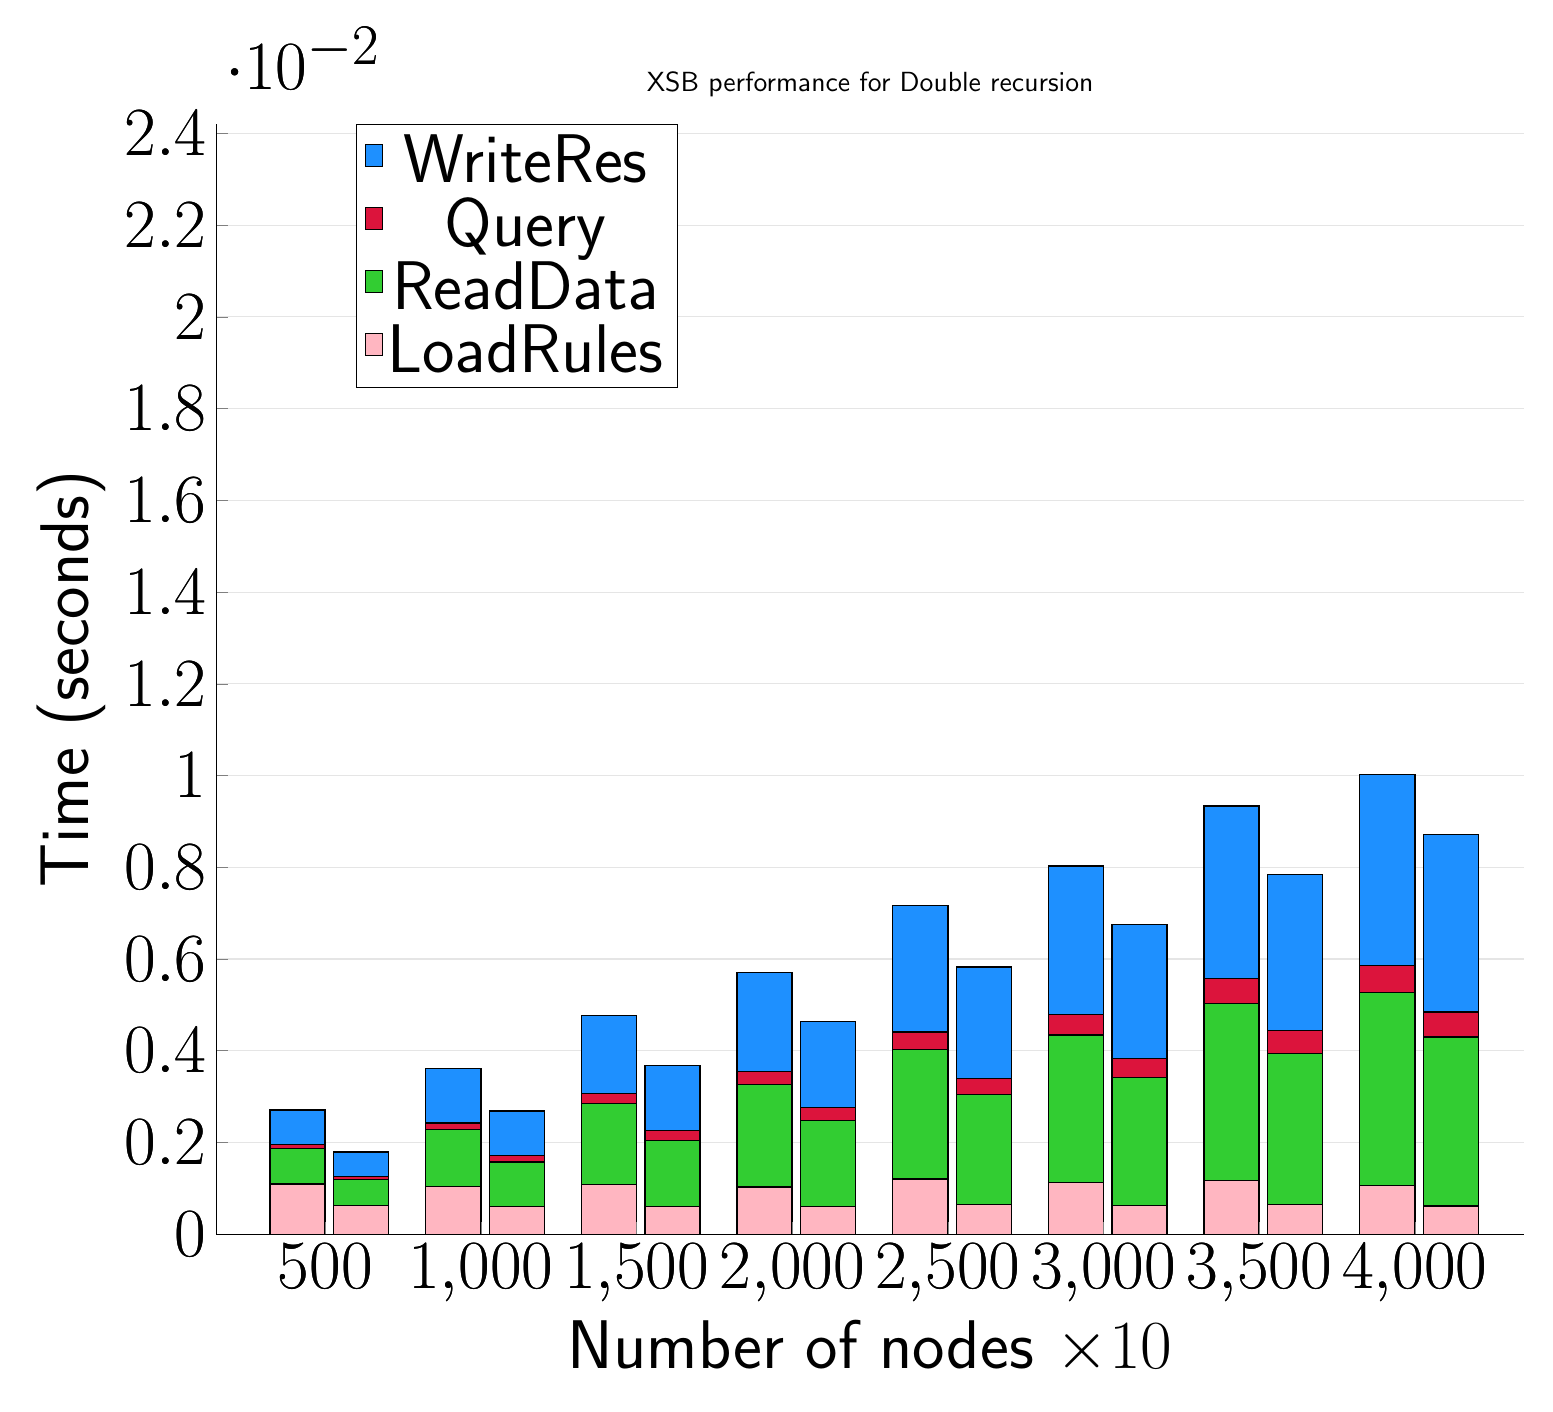
\begin{tikzpicture}
	\begin{axis}[
			ybar stacked,
			title={XSB performance for Double recursion},
			bar shift=-10pt,
			width=1.5\textwidth,
			bar width=0.7cm,
			ymajorgrids, tick align=inside,
			major grid style={draw=gray!20},
			xtick=data,
			ymin=0, ymax=0.024215764999389648,
			axis x line*=bottom,
			axis y line*=left,
			enlarge x limits=0.1,
			legend style={
					at={(0.23, 1)},
					anchor=north,
					legend columns=1,
					font=\Huge,
				},
			ylabel={Time (seconds)},
			xlabel={Number of nodes $\times 10$},
			label style={font=\Huge},
			tick label style={font=\Huge},
		]
		\addlegendimage{fill=DodgerBlue, draw=black, line width=0.2pt}
		\addlegendentry{WriteRes}
		\addlegendimage{fill=Crimson, draw=black, line width=0.2pt}
		\addlegendentry{Query}
		\addlegendimage{fill=LimeGreen, draw=black, line width=0.2pt}
		\addlegendentry{ReadData}
		\addlegendimage{fill=LightPink, draw=black, line width=0.2pt}
		\addlegendentry{LoadRules}
		\addplot +[fill=LightPink, draw=black, line width=0.5pt] coordinates {
				(500, 0.0010958194732666009)
				(1000, 0.0010375976562500007)
				(1500, 0.001082706451416016)
				(2000, 0.001030755043029783)
				(2500, 0.001206469535827636)
				(3000, 0.001129579544067382)
				(3500, 0.001173281669616699)
				(4000, 0.0010563611984252938)
			};
		\addplot +[fill=LimeGreen, draw=black, line width=0.5pt] coordinates {
				(500, 0.0007688283920288087)
				(1000, 0.0012402057647705072)
				(1500, 0.0017642498016357422)
				(2000, 0.0022292137145996102)
				(2500, 0.002824115753173827)
				(3000, 0.0032157897949218737)
				(3500, 0.003860044479370118)
				(4000, 0.004215764999389649)
			};
		\addplot +[fill=Crimson, draw=black, line width=0.5pt] coordinates {
				(500, 8.614063262939455e-05)
				(1000, 0.00015101432800292968)
				(1500, 0.0002269744873046875)
				(2000, 0.0002928972244262697)
				(2500, 0.0003762245178222654)
				(3000, 0.0004467010498046875)
				(3500, 0.0005407094955444337)
				(4000, 0.000589156150817871)
			};
		\addplot +[fill=DodgerBlue, draw=black, line width=0.5pt] coordinates {
				(500, 0.0007567405700683592)
				(1000, 0.0011876821517944342)
				(1500, 0.0016892671585083015)
				(2000, 0.0021589994430541992)
				(2500, 0.0027664899826049805)
				(3000, 0.003239631652832032)
				(3500, 0.003763842582702637)
				(4000, 0.004163384437561035)
			};
	\end{axis}
	\begin{axis}[
			ybar stacked,
			bar shift=13pt,
			width=1.5\textwidth,
			bar width=0.7cm,
			ymajorgrids, tick align=inside,
			major grid style={draw=none},
			xtick=data,
			ymin=0, ymax=0.024215764999389648,
			axis x line*=none,
			axis y line*=none,
			enlarge x limits=0.1,
			label style={font=\Huge},
			tick label style={font=\Huge},
		]
		\addplot +[fill=LightPink, draw=black, line width=0.5pt] coordinates {
				(500, 0.0006322000000000002)
				(1000, 0.0005981000000000004)
				(1500, 0.0006065999999999999)
				(2000, 0.0006004000000000002)
				(2500, 0.0006501)
				(3000, 0.0006298999999999999)
				(3500, 0.0006483000000000002)
				(4000, 0.0006143999999999996)
			};
		\addplot +[fill=LimeGreen, draw=black, line width=0.5pt] coordinates {
				(500, 0.0005545000000000002)
				(1000, 0.0009797)
				(1500, 0.0014429)
				(2000, 0.0018847000000000002)
				(2500, 0.0023991000000000004)
				(3000, 0.0027885999999999996)
				(3500, 0.0032934000000000006)
				(4000, 0.0036812)
			};
		\addplot +[fill=Crimson, draw=black, line width=0.5pt] coordinates {
				(500, 7.79e-05)
				(1000, 0.0001415999999999998)
				(1500, 0.0002112999999999995)
				(2000, 0.0002722000000000004)
				(2500, 0.00034920000000000025)
				(3000, 0.0004187999999999997)
				(3500, 0.0005028000000000001)
				(4000, 0.0005529000000000005)
			};
		\addplot +[fill=DodgerBlue, draw=black, line width=0.5pt] coordinates {
				(500, 0.0005295000000000003)
				(1000, 0.0009634000000000002)
				(1500, 0.0014229000000000004)
				(2000, 0.0018836999999999999)
				(2500, 0.0024296)
				(3000, 0.0029121)
				(3500, 0.0034002)
				(4000, 0.003871899999999999)
			};
	\end{axis}
\end{tikzpicture}

\end{document}
